\documentclass[a4paper]{article}
\usepackage{import}
\usepackage[utf8]{inputenc}
\usepackage[T1]{fontenc}
\usepackage{textcomp}
\usepackage[italian]{babel}
\usepackage{amsmath, amssymb}
\usepackage{booktabs,xltabular}
\usepackage{amsfonts}
\usepackage{subcaption}
\usepackage{amsthm}
\usepackage{cancel}
\usepackage{mdframed}
\usepackage{makecell}
\usepackage{float}
\usepackage{xcolor}
\usepackage{listings}
\usepackage{gensymb}
\usepackage{graphicx}
\usepackage{bodeplot}
\usepackage{physics}
\usepackage{tikz}
\usetikzlibrary{shapes, arrows, automata, petri, decorations.markings, decorations.pathreplacing, positioning, calc, quotes}
\usepackage{circuitikz}
\usepackage[label=corner]{karnaugh-map}
\graphicspath{{./figures/}}

% Set default font to sans-serif
\renewcommand{\familydefault}{\sfdefault} 
\usepackage{eulervm}

\usepackage{forest}

\usepackage{mathtools}
\DeclarePairedDelimiter\ceil{\lceil}{\rceil}
\DeclarePairedDelimiter\floor{\lfloor}{\rfloor}

% \usepackage{ntheorem}

\usepackage{import}
\usepackage{pdfpages}
\usepackage{transparent}
\usepackage{xcolor}

\usepackage{hyperref}
\hypersetup{
    colorlinks=false,
}

% Code blocks
\definecolor{codegreen}{rgb}{0,0.6,0}
\definecolor{codegray}{rgb}{0.5,0.5,0.5}
\definecolor{codepurple}{rgb}{0.58,0,0.82}
\definecolor{backcolour}{rgb}{0.95,0.95,0.95}

\lstdefinestyle{mystyle}{
	backgroundcolor=\color{backcolour},
	commentstyle=\color{codegreen},
	keywordstyle=\color{magenta},
	numberstyle=\tiny\color{codegray},
	stringstyle=\color{codepurple},
	basicstyle=\ttfamily\footnotesize,
	breakatwhitespace=false,
	breaklines=true,
	captionpos=b,
	keepspaces=true,
	numbers=left,
	numbersep=5pt,
	showspaces=false,
	showstringspaces=false,
	showtabs=false,
	tabsize=2
}

\lstset{style=mystyle}

\usepackage{color}
\usepackage{import}
\usepackage{pdfpages}
\usepackage{transparent}
\usepackage{xcolor}

% Example frame
\theoremstyle{definition}
\newmdtheoremenv[%
	linecolor=gray,leftmargin=0,%
	rightmargin=0,
	innertopmargin=8pt,%
	innerbottommargin=8pt,
	ntheorem]{example}{Esempio}[section]

% Important definition frame
\theoremstyle{definition}
\newmdtheoremenv[%
	linecolor=gray,leftmargin=0,%
	rightmargin=0,
	backgroundcolor=gray!40,%
	innertopmargin=8pt,%
	innerbottommargin=8pt,
	ntheorem]{definition}{Definizione}[section]

% Exercise frame
\theoremstyle{definition}
\newmdtheoremenv[%
	linecolor=gray,leftmargin=0,%
	rightmargin=0,
	innertopmargin=8pt,%
	innerbottommargin=8pt,
	ntheorem]{exercise}{Esercizio}[section]

% Theorem frame
\theoremstyle{definition}
\newmdtheoremenv[%
  linecolor=gray,leftmargin=0,%
  rightmargin=0,
  innertopmargin=8pt,%
  innerbottommargin=8pt,
  ntheorem]{theorem}{Teorema}[section]

\theoremstyle{definition}
\newmdtheoremenv[%
  linecolor=white,leftmargin=0,%
  rightmargin=0,
  innertopmargin=8pt,%
  innerbottommargin=8pt,
  ntheorem]{define}{Definizione utile}[section]

% figure support
\usepackage{import}
\usepackage{xifthen}
\pdfminorversion=7
\usepackage{pdfpages}
\usepackage{transparent}
\newcommand{\incfig}[1]{%
	\def\svgwidth{\columnwidth}
	\import{./figures/}{#1.pdf_tex}
}

% FSM tikz
\tikzset{
    place/.style={
        circle,
        thick,
        draw=black,
        minimum size=6mm,
    },
        state/.style={
        circle,
        thick,
        draw=black,
        fill=white,
        minimum size=6mm,
    },
}

\pdfsuppresswarningpagegroup=1

\usepackage{pgfplots}
\pgfplotsset{compat=1.18,width=10cm}

% Save plots as pdf and reuse them without compiling every time
\usetikzlibrary{external}
\tikzexternalize[prefix=figures/tikz/, optimize=false]


\begin{document}

\begin{titlepage}
	\begin{center}
		\vspace*{1cm}

		\Huge
		\textbf{Probabilità e Statistica\\Esercizi}

		\vspace{0.5cm}
		\LARGE
		UniVR - Dipartimento di Informatica

		\vspace{1.5cm}

		\textbf{Fabio Irimie}

		\vfill


		\vspace{0.8cm}


		2° Semestre 2023/2024

	\end{center}
\end{titlepage}


\tableofcontents
\pagebreak

\section{Indirizzamento}
\subsection{Esercizio 1}
Qual'è l'indirizzo di rete se ho il seguente indirizzo IP:
\[
  140.120.84.20/20
\] 

\subsubsection{Risoluzione}
L'indirizzo di rete corrisponde ai primi 20 bit dell'indirizzo IP, quindi bisogna
passare alla notazione binaria:
\[
  140.120.84.20 \to 10001100 \;\; 01111000 \;\; 01010100 \;\; 00010100
\] 
I primi 20 bit sono assegnati al prefisso:
\[
  \underbrace{10001100 \;\; 01111000 \;\; 0101}_{\text{Prefisso}} \;\;
  \underbrace{0100 \;\; 00010100}_{\text{Suffisso}}
\] 
Per ottenere l'indirizzo di rete bisogna azzerare i bit del suffisso:
\[
  \underbrace{10001100 \;\; 01111000 \;\; 0101}_{\text{Prefisso}} \;\;
  \underbrace{0000 \;\; 00000000}_{\text{Suffisso}}
\] 
che in notazione decimale puntata diventa:
\[
  140.120.80.0
\] 
La maschera di questo IP è:
\[
  \underbrace{11111111 \;\; 11111111 \;\; 1111}_{\text{Prefisso}} \;\;
  \underbrace{0000 \;\; 00000000}_{\text{Suffisso}}
\] 
che in notazione decimale puntata diventa:
\[
  255.255.240.0
\] 

\subsection{Esercizio 2}
Si hanno 3 LAN. All'insieme delle 3 LAN è stato assegnato il blocco:
\[
  165.5.1.0/24
\] 
Creare 3 sottoreti per le 3 LAN in modo che abbiano tutte lo stesso numero di host.

\subsubsection{Risoluzione}
Per prima cosa si trasforma l'indirizzo IP in notazione binaria:
\[
  \underbrace{1010 0101 \;\; 0000 0101 \;\; 0000 0001}_{\text{Prefisso}} \;\;
  \underbrace{0000 0000}_{\text{Suffisso}}
\] 
Per poter ottenere 3 sottoreti di dimensione servono 2 bit che vengoo presi dal suffisso
per identificare ciascuna delle 3 reti:
\[
  \underbrace{1010 0101 \;\; 0000 0101 \;\; 0000 0001}_{\text{Prefisso}} \;
  \underbrace{00}_{\text{Sottorete}} \;
  \underbrace{00 0000}_{\text{Suffisso}}
\] 
Le combinazioni possibili sono:
\begin{itemize}
  \item 
    \(
    \underbrace{1010 0101 \;\; 0000 0101 \;\; 0000 0001}_{\text{Prefisso}} \;
    \underbrace{00}_{\text{Sottorete}} \;
    \underbrace{00 0000}_{\text{Suffisso}}
    \) 

  \item 
    \(
    \underbrace{1010 0101 \;\; 0000 0101 \;\; 0000 0001}_{\text{Prefisso}} \;
    \underbrace{01}_{\text{Sottorete}} \;
    \underbrace{00 0000}_{\text{Suffisso}}
    \) 

  \item 
    \(
    \underbrace{1010 0101 \;\; 0000 0101 \;\; 0000 0001}_{\text{Prefisso}} \;
    \underbrace{10}_{\text{Sottorete}} \;
    \underbrace{00 0000}_{\text{Suffisso}}
    \) 

  \item 
    \(
    \underbrace{1010 0101 \;\; 0000 0101 \;\; 0000 0001}_{\text{Prefisso}} \;
    \underbrace{11}_{\text{Sottorete}} \;
    \underbrace{00 0000}_{\text{Suffisso}}
    \) 
\end{itemize}
Ci troviamo con 4 sottoreti con lo stesso numero di indirizzi \( \left( 2^6 = 64 \right) \).
Di queste 4 sottoreti ne utilizziamo 3 e l'ultima rimane libera per utilizzi futuri.

\vspace{1em}
\noindent
Traducendo i blocchi in notazione decimale puntata si ha:
\[
  \begin{aligned}
    165.5.1.0/26 \to \text{LAN 1}\\
    165.5.1.64/26 \to \text{LAN 2}\\
    165.5.1.128/26 \to \text{LAN 3}\\
    165.5.1.192/26 \to \text{Libero}
  \end{aligned}
\] 

\subsection{Esercizio 3}
Usando lo stesso blocco dell'esercizio 2 si modifichi la LAN 1 affinchè abbia il doppio
degli indirizzi rispetto a quelli assegnati alle altre 2 LAN.

\subsubsection{Risoluzione}
Il blocco di partenza in notazione binaria è:
\[
  10100101 \;\; 00000101 \;\; 00000001 \;\; 00000000
\] 
Per ottenere il doppio degli indirizzi rispetto alle altre 2 LAN bisogna prendere un bit
dal suffisso e assegnarlo al prefisso ottenendo così 2 reti /25.
\[
  \begin{aligned}
    \underbrace{1010 0101 \;\; 0000 0101 \;\; 0000 0001}_{\text{Prefisso}} \;
    \underbrace{0}_{\text{Sottorete}} \;
    \underbrace{000 0000}_{\text{Suffisso}}\\
    \underbrace{1010 0101 \;\; 0000 0101 \;\; 0000 0001}_{\text{Prefisso}} \;
    \underbrace{1}_{\text{Sottorete}} \;
    \underbrace{000 0000}_{\text{Suffisso}}
  \end{aligned}
\]
Dalla rete si fa la stessa operazione separando un bit dal suffisso e ottenendo altri 
2 blocchi da /26.
\[
\begin{aligned}
    \underbrace{1010 0101 \;\; 0000 0101 \;\; 0000 0001}_{\text{Prefisso}} \;
    \underbrace{0}_{\text{Lan 1}} \;
    \underbrace{000 0000}_{\text{Suffisso}}\\
    \underbrace{1010 0101 \;\; 0000 0101 \;\; 0000 0001}_{\text{Prefisso}} \;
    \underbrace{10}_{\text{Lan 2}} \;
    \underbrace{00 0000}_{\text{Suffisso}}\\
    \underbrace{1010 0101 \;\; 0000 0101 \;\; 0000 0001}_{\text{Prefisso}} \;
    \underbrace{11}_{\text{Lan 3}} \;
    \underbrace{00 0000}_{\text{Suffisso}}
\end{aligned}
\] 
Traducendo i blocchi in notazione decimale puntata si ha:
\[
  \begin{aligned}
    \text{Lan 1: } & 165.5.1.0/25\\
    \text{Lan 2: } & 165.5.1.128/26\\
    \text{Lan 3: } & 165.5.1.192/26
  \end{aligned}
\] 

\subsection{Esercizio 4}
Si consideri la seguente rete suddivisa in 5 sottoreti:
\begin{figure}[H]
  \centering
  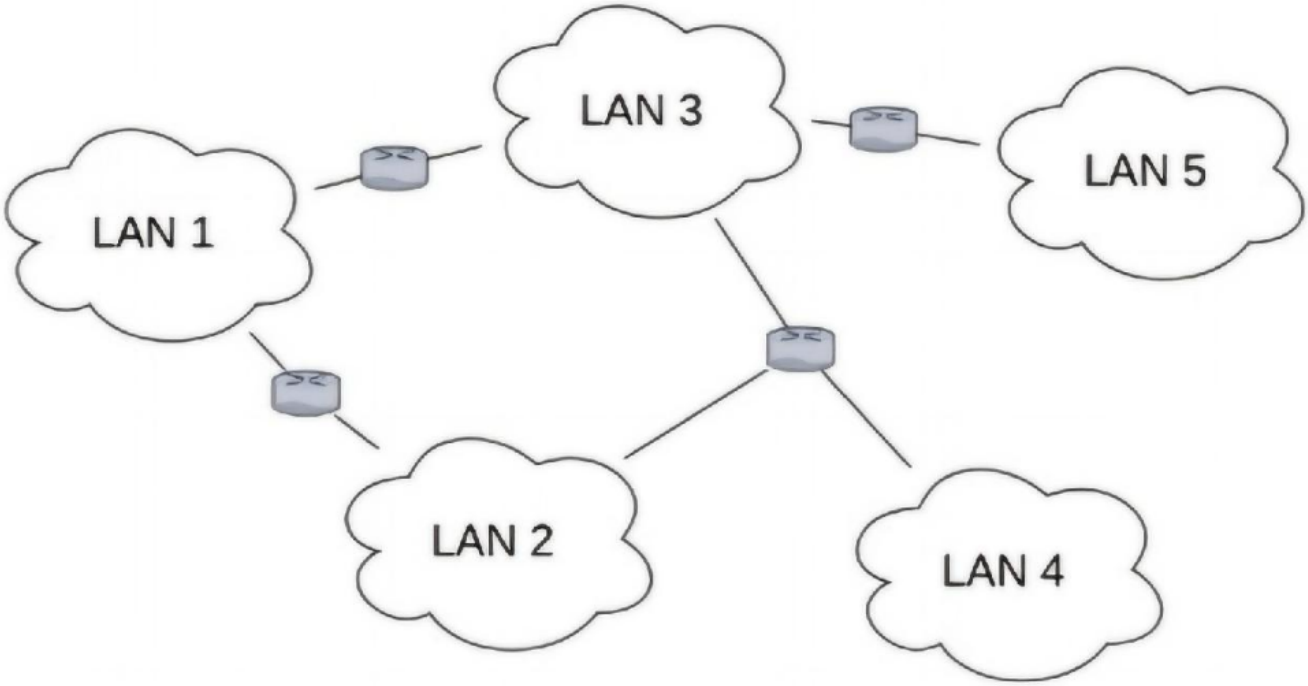
\includegraphics[width=0.75\textwidth]{../figures/esercitazione-es1}
\end{figure}

\noindent
Ci sono due indirizzi già assegnati alla rete:
\begin{itemize}
  \item 101.75.79.255
  \item 101.75.80.0
\end{itemize}

\begin{enumerate}
  \item Qual'è il blocco \textbf{CIDR} più piccolo (con il minor numero di indirizzi) che
    contiene tali indirizzi?
  \item Dato il blocco \textbf{CIDR} della domanda precedente, si creino 5 sottoreti con
    i seguenti vincoli:
\begin{itemize}
  \item \textbf{LAN 1}: deve essere una sottorete /21

  \item \textbf{LAN 2}: deve ospitare fino a 1000 host

  \item \textbf{LAN 3}: deve essere una sottorete /23
  \item \textbf{LAN 4}: deve ospitare fino a 400 host

  \item \textbf{LAN 5}: deve ospitare metà host rispetto al blocco iniziale
\end{itemize}
\end{enumerate}

\subsubsection{Risoluzione}
\begin{enumerate}
  \item 
    Converto entrambi gli indirizzi in notazione binaria:
    \[
      \begin{aligned}
        101.75.79.255 & \to 01100101 \;\; 01001011 \;\; 01001111 \;\; 11111111 \\
        101.75.80.0   & \to 01100101 \;\; 01001011 \;\; 01010000 \;\; 00000000
      \end{aligned}
    \] 
    Siccome i due IP sono uguali fino al 19° bit a partire da sinistra, si può dire che
    il blocco CIDR più piccolo che contiene entrambi gli indirizzi sia quello della rete:
    \[
      \underbrace{01100101 \;\; 01001011 \;\; 010}_{\text{Prefisso}}
      \;\; \underbrace{00000 \;\; 00000000}_{\text{Suffisso}}
    \]
    che in notazione intera puntata è il seguente:
    \[
      101.75.64.0/19
    \] 

  \item 
    \begin{itemize}
      \item \textbf{LAN 1}:

    \vspace{1em}
    \noindent
    Per avere una sottorete /21 basta spostare i bit del prefisso:
    \[
      \underbrace{01100101 \;\; 01001011 \;\; 010}_{\text{Prefisso}}
      \;\; \underbrace{00000 \;\; 00000000}_{\text{Suffisso}}\\
    \]
    \[
      \Downarrow
    \]
    \[
      \underbrace{01100101 \;\; 01001011 \;\; 01000}_{\text{Prefisso}}
      \;\; \underbrace{000 \;\; 00000000}_{\text{Suffisso}}\\
    \] 
    che in notazione intera puntata risulta:
    \[
      101.75.64.0/21
    \] 

  \item \textbf{LAN 2}:

    \vspace{1em}
    \noindent
    1000 host sono circa \( 2^{10} \), di conseguenza per avere un blocco che possa
    ospitare fino a 1000 host esso deve avere almeno 10 bit di suffisso:
    \[
      \underbrace{01100101 \;\; 01001011 \;\; 010000}_{\text{Prefisso}}
      \;\; \underbrace{00 \;\; 00000000}_{\text{Suffisso}}\\
    \] 
    che in notazione intera puntata risulta:
    \[
      101.75.64.0/22
    \] 

  \item \textbf{LAN 3}:

    \vspace{1em}
    \noindent
    Per avere una sottorete /23 basta spostare i bit del prefisso:
    \[
      \underbrace{01100101 \;\; 01001011 \;\; 010}_{\text{Prefisso}}
      \;\; \underbrace{00000 \;\; 00000000}_{\text{Suffisso}}\\
    \]
    \[
      \Downarrow
    \]
    \[
      \underbrace{01100101 \;\; 01001011 \;\; 0100000}_{\text{Prefisso}}
      \;\; \underbrace{0 \;\; 00000000}_{\text{Suffisso}}\\
    \] 
    che in notazione intera puntata risulta:
    \[
      101.75.64.0/23
    \] 


  \item \textbf{LAN 4}:

    \vspace{1em}
    \noindent
    400 host sono circa \( 2^{9} \), di conseguenza per avere un blocco che possa
    ospitare fino a 400 host esso deve avere almeno 9 bit di suffisso:
    \[
      \underbrace{01100101 \;\; 01001011 \;\; 0100000}_{\text{Prefisso}}
      \;\; \underbrace{0 \;\; 00000000}_{\text{Suffisso}}\\
    \] 
    che in notazione intera puntata risulta:
    \[
      101.75.64.0/23
    \] 

  \item \textbf{LAN 5}:

    \vspace{1em}
    \noindent
    Il blocco iniziale riesce ad ospitare \( 2^{13} \) host, quindi per creare una rete
    che ne ospiti la metà bisogna avere \( \frac{2^{13}}{2} = 2^{13-1} = 2^{12} \) 12
    bit di suffisso:
    \[
      \underbrace{01100101 \;\; 01001011 \;\; 0100}_{\text{Prefisso}}
      \;\; \underbrace{0000 \;\; 00000000}_{\text{Suffisso}}\\
    \] 
    che in notazione intera puntata risulta:
    \[
      101.75.64.0/20
    \] 
\end{itemize}
\end{enumerate}

\subsection{Esercizio 5}
Si hanno 3 LAN con i seguenti numeri di host:
\begin{enumerate}
  \item LAN 1: 300 host
  \item LAN 2: 40 host
  \item LAN 3: 90 host
\end{enumerate}
L'indirizzo di broadcast della LAN 3 è:
\[
148.12.79.255
\] 
\begin{enumerate}
  \item Trovare il blocco CIDR totale da assegnare all'intera rete
  \item Partendo da tale blocco suddividerlo in sottoreti da assegnare alle 3 LAN
\end{enumerate}

\subsubsection{Risoluzione}
\begin{enumerate}
  \item 
    Per trovare il blocco CIDR totale bisogna trovare il blocco che riesce a contenere
    il numero di host totale (in base 2) delle 3 LAN:
    \[
      512 + 64 + 128 = 704
    \] 
    Il blocco CIDR che riesce a contenere 704 host è:
    \[
      2^{10} = 1024
    \] 
    Di conseguenza il blocco CIDR totale dovrà avere 10 bit di suffisso e l'indirizzo di
    rete si ottiene convertendo l'indirizzo di broadcast in notazione binaria e azzerando
    i bit del suffisso:
    \[
      \underbrace{1001 0100 \;\; 0000 1100 \;\; 0100 11}_{\text{Prefisso}}
      \;\; \underbrace{00 \;\; 00000000}_{\text{Suffisso}}
    \] 
    che in decimale risulta:
    \[
      148.12.76.0/22
    \] 

  \item 
    Per suddividere il blocco CIDR in 3 sottoreti bisogna trovare il numero di bit di
    suffisso necessari per contenere il numero di host di ciascuna LAN:
    \begin{itemize}
      \item LAN 1: 300 host, \( 2^9 = 512 \) quindi 9 bit di suffisso
      \item LAN 2: 40 host, \( 2^6 = 64 \) quindi 6 bit di suffisso
      \item LAN 3: 90 host, \( 2^7 = 128 \) quindi 7 bit di suffisso
    \end{itemize}
    Quindi il blocco CIDR totale:
    \[
      \underbrace{1001 0100 \;\; 0000 1100 \;\; 0100 11}_{\text{Prefisso}}
      \;\; \underbrace{00 \;\; 00000000}_{\text{Suffisso}}
    \] 
    verrà suddiviso in:
    \[
      \begin{aligned}
        \text{LAN 1: } &
        \underbrace{1001 0100 \;\; 0000 1100 \;\; 0100 11}_{\text{Prefisso}}
        \;\; \underbrace{0}_{\text{Lan 1}}
        \;\; \underbrace{0\;\;00000000}_{\text{Suffisso}}\\
        \text{LAN 2: } &
        \underbrace{1001 0100 \;\; 0000 1100 \;\; 0100 11}_{\text{Prefisso}}
        \;\; \underbrace{11\;\;01}_{\text{Lan 2}}
        \;\; \underbrace{000000}_{\text{Suffisso}}\\
        \text{LAN 3: } &
        \underbrace{1001 0100 \;\; 0000 1100 \;\; 0100 11}_{\text{Prefisso}}
        \;\; \underbrace{11\;\;1}_{\text{Lan 3}}
        \;\; \underbrace{0000000}_{\text{Suffisso}}\\
      \end{aligned}
    \]
    che in notazione puntata risultano:
    \[
    \begin{aligned}
      \text{LAN 1: } & 148.12.76.0/23\\
      \text{LAN 2: } & 148.12.79.64/26\\
      \text{LAN 3: } & 148.12.79.128/25
    \end{aligned}
    \] 
\end{enumerate}

\subsection{Esercizio 6}
Si hanno 4 lan che devono contenere il seguente numero di host:
\[
\begin{aligned}
  \text{LAN 1: } & 130 \, host\\
  \text{LAN 2: } & 270 \, host\\
  \text{LAN 3: } & 65 \, host\\
  \text{LAN 4: } & 35 \, host\\
\end{aligned}
\] 
La LAN 1 contiene l'indirizzo 46.144.141.41.
\begin{enumerate}
  \item Calcolare il blocco CIDR totale.
  \item Quali sono gli indirizzi di rete delle 4 LAN?
\end{enumerate}

\subsubsection{Risoluzione}
\begin{enumerate}
  \item 
    Per trovare il blocco CIDR totale bisogna trovare il blocco di indirizzi che
    contiene tutti gli indirizzi delle LAN (in base 2):
    \[
      \begin{aligned}
        \text{LAN 1: } & 130 \to 256 = 2^8\\
        \text{LAN 2: } & 270 \to 512 = 2^9\\
        \text{LAN 3: } & 65 \to 128 = 2^7\\
        \text{LAN 4: } & 35 \to 64 = 2^6
      \end{aligned}
    \] 
    il blocco totale sarà:
    \[
      256 + 512 + 128 + 64 = 960 \to 1024 = 2^{10}
    \] 
    Avremo bisogno di 10 bit per il suffisso per poter indirizzare \( 1024 \) host.

    \vspace{1em}
    \noindent
    Convertiamo l'indirizzo contenuto dalla LAN 1 in binario per poter ricavare l'indirizzo
    di rete:
    \[
      46.144.141.41
    \] 
    \[
      \downarrow
    \] 
    \[
      00101110 \;\; 10010000 \;\; 10001101 \;\; 00101001
    \] 
    Sappiamo che 10 bit vanno dedicati al suffisso, di conseguenza 22 saranno dedicati al
    prefisso, quindi l'indirizzo di rete è: 
    \[
      \underbrace{00101110 \;\; 10010000 \;\; 100011}_{\text{Prefisso}}
      \underbrace{00 \;\; 00000000}_{\text{Suffisso}}
    \] 
    che in notazione decimale diventa:
    \[
      46.144.140.0/22
    \] 

  \item Per trovare gli indirizzi di ognuna delle LAN dobbiamo vedere quanti bit bisogna
    assegnare ad ognuna di esse per indirizzare tutti gli host richiesti. Abbiamo visto
    nella domanda precedente che gli indirizzi richiesti per ogni lan sono i seguenti:
    \[
      \begin{aligned}
        \text{LAN 1: } & 130 \to 256 = 2^8\\
        \text{LAN 2: } & 270 \to 512 = 2^9\\
        \text{LAN 3: } & 65 \to 128 = 2^7\\
        \text{LAN 4: } & 35 \to 64 = 2^6
      \end{aligned}
    \] 
    \begin{itemize}
      \item La LAN 1 richiede 8 bit di suffisso e sappiamo che contiene il seguente
        indirizzo:
        \[
          \underbrace{00101110 \;\; 10010000 \;\; 100011}_{\text{Prefisso}}
          \underbrace{01}_{\text{LAN 1}}
          \underbrace{00101001}_{\text{Suffisso}}
        \] 
        di conseguenza l'indirizzo di rete della LAN 1 è:
        \[
          \underbrace{00101110 \;\; 10010000 \;\; 100011}_{\text{Prefisso}}
          \underbrace{01}_{\text{LAN 1}}
          \underbrace{00000000}_{\text{Suffisso}}
        \] 
        \[
          \downarrow
        \] 
        \[
          46.144.141.0/24
        \] 
      \item La LAN 2 richiede 9 bit di suffisso:
        \[
          \underbrace{00101110 \;\; 10010000 \;\; 100011}_{\text{Prefisso}}
          \underbrace{1}_{\text{LAN 2}}
          \underbrace{0 \;\; 00000000}_{\text{Suffisso}}
        \] 
        \[
          \downarrow
        \] 
        \[
          46.144.142.0/23
        \] 
      \item La LAN 3 richiede 7 bit di suffisso:
        \[
          \underbrace{00101110 \;\; 10010000 \;\; 100011}_{\text{Prefisso}}
          \underbrace{00 \;\; 1}_{\text{LAN 3}}
          \underbrace{0000000}_{\text{Suffisso}}
        \] 
        \[
          \downarrow
        \] 
        \[
          46.144.140.128/25
        \] 
      \item La LAN 4 richiede 6 bit di suffisso:
        \[
          \underbrace{00101110 \;\; 10010000 \;\; 100011}_{\text{Prefisso}}
          \underbrace{00 \;\; 01}_{\text{LAN 4}}
          \underbrace{000000}_{\text{Suffisso}}
        \] 
        \[
          \downarrow
        \] 
        \[
          46.144.140.64/26
        \] 
    \end{itemize}
\end{enumerate}

\subsection{Esercizio 7}
Si hanno 3 lan con i seguenti host:
\[
\begin{aligned}
  \text{LAN 1: } & 400 \, host\\
  \text{LAN 2: } & 300 \, host\\
  \text{LAN 3: } & 1200 \, host
\end{aligned}
\] 
La LAN 1 contiene un host con indirizzo:
\[
178.242.85.168
\] 
Si consideri la topologia con un router di bordo \( X \)  tra la rete internet e la LAN1, un secondo
router di bordo \( A \)  tra la LAN1 e la LAN2, un terzo router di bordo \( B \)  tra la LAN2 e la LAN3
e un ultimo router di bordo \( D \) collegato alla LAN3 e al router di bordo della rete internet.

Ogni host è collegato tramite un cavo coassiale a tutti gli altri host e anche al router
e quindi li raggiunte entrambi con 1 hop.
\begin{enumerate}
  \item Calcolare il blocco CIDR totale.
  \item Calcolare gli indirizzi di rete delle 3 LAN.
  \item Trovare la tabella di routing del router \( A \) considerando come metrica
    il numero di hop e assumendo che il router \( X \) abbia annunciato di ragginugere
    tutti gli host su Internet con 5 hop.
\end{enumerate}

\section{TCP}
L'obiettivo di questi esercizi è quello di vedere come si comporta l'algoritmo in situazioni 
particolari.
\subsection{Esercizio 1}
Un'applicazione \( A \) deve trasferire verso un'applicazione \( B \) \( 96000 byte \).
Si suppone che la connessione sia già stata instaurata. I dati sono i seguenti:
\begin{itemize}
  \item \texttt{mss} = 1000 byte
  \item \texttt{rcvwnd} = 32000 byte, costante per l'intero trasferimento dei dati
  \item \texttt{ssthresh} = \( \frac{\texttt{rcvwnd}_{\text{iniziale}}}{2} \) 
  \item \texttt{rtt} = costante, pari a \( 0.5 \) secondi
  \item \texttt{rto} = \( 2 \cdot \texttt{rtt} \), raddoppia in caso di perdite sequenziali
  \item Down di rete (rete fuori uso, in cui tutti i segmenti vengono persi) = 
    \[
    \begin{aligned}
      t_1 = 3 &\to t_2 = 3,5\\
      t_3 = 7 &\to t_4 = 7,5
    \end{aligned}
    \] 
\end{itemize}
Lo scopo è quello di valutare l'evoluzione temporale della \texttt{cwnd} fino a fine
trasmissione.

\subsubsection{Risoluzione}
Il numero di segmenti da trasmettere sono:
\[
  \frac{\text{byte da trasmettere}}{\text{\texttt{mss}}} = \frac{96000 byte}{1000 byte}
  = 96 \text{ segmenti}
\] 
La \texttt{rcvwnd} iniziale vale:
\[
  \text{\texttt{rcvwnd}}_{\text{iniziale}} = \frac{32000 byte}{1000 byte} = 32 \text{ segmenti}
\] 
La \texttt{ssthresh} vale:
\[
  \text{\texttt{ssthresh}}_{\text{iniziale}} = \frac{32}{2} = 16 \text{ segmenti}
\]
La \texttt{cwnd} iniziale vale 1:
\[
  \text{\texttt{cwnd}}_{\text{iniziale}} = 1
\] 

\vspace{1em}
\noindent
L'andamento della trasmissione è il seguente:
\begin{figure}[H]
  \centering
  \begin{tikzpicture}
    \draw[->] (0,-0.2) -- (0,10.5) node[left] {\( w \)};
    \draw[->] (-0.2,0) -- (10.5,0) node[below] {\( t \)};

    % rcvwnd & ssthresh
    \draw[orange] (0,16/2) node[above right] {\texttt{ssthresh}} -- (8/2,16/2)
      -- (8/2,9/2) -- (16/2,9/2)
      -- (16/2,5/2) -- (20/2,5/2);

    % Down
    \fill[red,opacity=0.2] (6/2,0) rectangle (7/2,10.5);
    \fill[red,opacity=0.2] (14/2,0) rectangle (15/2,10.5);

    \fill[blue] (0,1/2) circle (0.05);
    \fill[blue] (1/2,2/2) circle (0.05);
    \fill[blue] (2/2,4/2) circle (0.05);
    \fill[blue] (3/2,8/2) circle (0.05);
    \fill[blue] (4/2,16/2) circle (0.05);
    \fill[blue] (5/2,17/2) circle (0.05);
    \fill[blue] (6/2,18/2) circle (0.05) node[right,red] {\( \times \)};
    \draw[blue] (0,1/2) -- (1/2,2/2) -- (2/2,4/2) -- (3/2,8/2) -- (4/2,16/2)
      -- (5/2,17/2) -- (6/2,18/2);

    % Loss
    \draw[purple,dashed] (3.5,18/2) -- (4,18/2) node[above] {\texttt{RTO}} -- (4,1/2);

    \fill[blue] (8/2,1/2) circle (0.05);
    \fill[blue] (9/2,2/2) circle (0.05);
    \fill[blue] (10/2,4/2) circle (0.05);
    \fill[blue] (11/2,8/2) circle (0.05);
    \fill[blue] (12/2,9/2) circle (0.05);
    \fill[blue] (13/2,10/2) circle (0.05);
    \fill[blue] (14/2,11/2) circle (0.05) node[right,red] {\( \times \)};
    \draw[blue] (8/2,1/2) -- (9/2,2/2) -- (10/2,4/2) -- (11/2,8/2) -- (12/2,9/2)
      -- (13/2,10/2) -- (14/2,11/2);

    % Loss
    \draw[purple,dashed] (7.5,11/2) -- (8,11/2) -- (8,1/2);

    \fill[blue] (16/2,1/2) circle (0.05);
    \fill[blue] (17/2,2/2) circle (0.05);
    \fill[blue] (18/2,4/2) circle (0.05);
    \fill[blue] (19/2,5/2) circle (0.05);
    \fill[blue] (20/2,6/2) circle (0.05);
    \draw[blue] (16/2,1/2) -- (17/2,2/2) -- (18/2,4/2) -- (19/2,5/2) -- (20/2,6/2);

    % Ticks
    \foreach \x in {1,2,3,4,5,6,7,8,9,10,11,12,13,14,15,16,17,18,19,20}
    \draw (\x/2,-0.1) -- (\x/2,0.1);

    \foreach \y in {1,2,3,4,5,6,7,8,9,10,11,12,13,14,15,16,17,18,19,20}
    \draw (0,\y/2) -- (0.1,\y/2);

    \foreach \y in {1,2,4,8,16}
    \draw (-0.1,\y/2) -- (0.1,\y/2) node[left=0.2] {\y};

    \node[below,scale=0.6] at (0.5,0) {0.5};
    \node[below,scale=0.6] at (1,-0.1) {1};
    \node[below,scale=0.6] at (3,-0.1) {3};
    \node[below,scale=0.6] at (3.5,-0.1) {3.5};
    \node[below,scale=0.6] at (7,-0.1) {7};
    \node[below,scale=0.6] at (7.5,-0.1) {7.5};

    \draw[green!50!black] (0.05,-0.2) -- ++(0,-0.2) -- ++(0.45,0)
      node[midway,below] {RTT} -- ++(0,0.2);
  \end{tikzpicture}
  \caption{Andamento di \texttt{cwnd} in funzione del tempo}
\end{figure}
\noindent
Il numero di segmenti trasmessi è:
\[
  \#seg = 1 + 2 + 4 + 8 + 16 + 17 + \cancel{18} + 1 + 2 + 4 + 8 + 9 + 10 + \cancel{11}
  + 1 + 2 + 4 + 5 + \stackrel{2}{\cancel{6}}
\] 
\[
  = 96
\] 
All'ultimo RTT si trasmettono soltanto 2 segmenti al posto di 6 perchè nonostante la 
finestra sia grande 6, il numero di pacchetti rimasti da trasmettere sono soltanto 2.

\vspace{1em}
\noindent
Un'altra possibile rappresentazione è la seguente:
\begin{figure}[H]
  \centering
  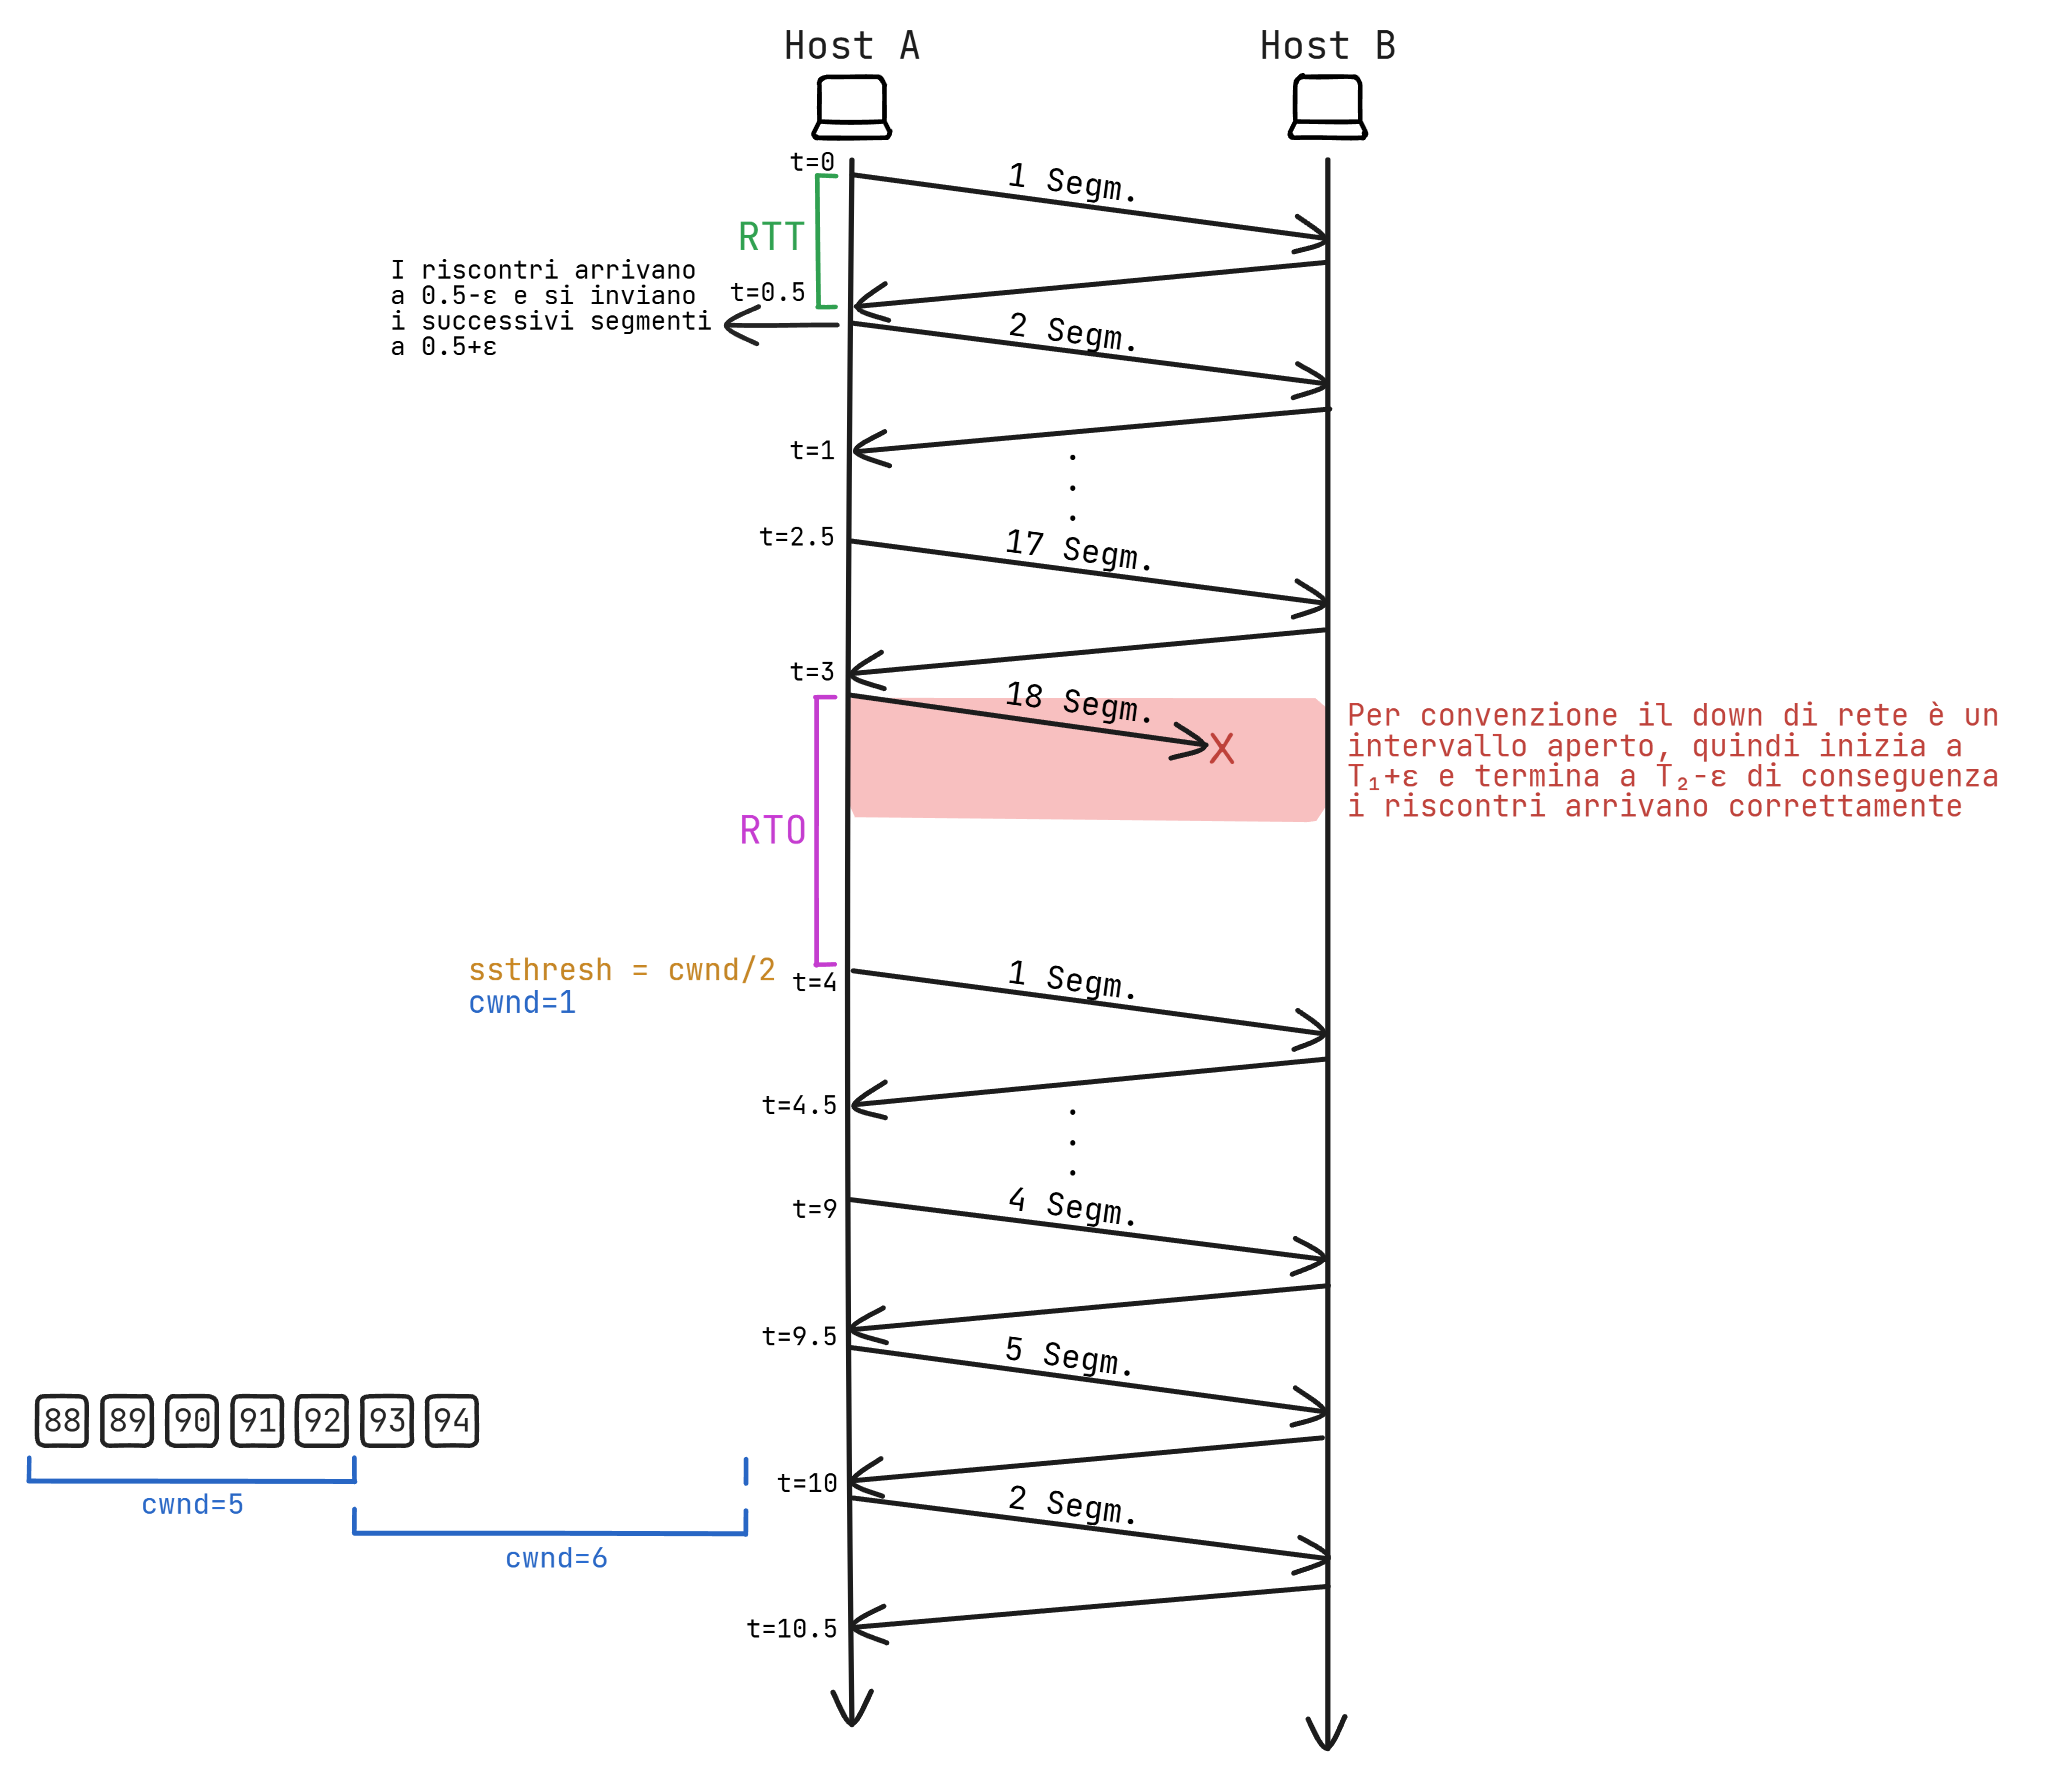
\includegraphics[width=1\textwidth]{../figures/es-tcp1}
\end{figure}


\subsection{Esercizio 2}
Abbiamo un'applicazione \( A \) che trasferisce \( 46500byte \) verso un'applicazione \( B \).
\[
\begin{aligned}
  MSS &= 1500 \text{ byte}\\
  RCVWND_{\text{iniziale}} &= 24000 \text{ byte} \to \text{ costante}\\
  SSTHRESH &= \frac{RCVWND_{\text{iniziale}}}{2}\\
  RTT &= 0.5 \text{ secondi} \to \text{ costante}\\
  RTO &= 2 \cdot RTT \to \text{ raddoppia in caso di perdite consecutive}\\
  \text{Down di rete} &= [1.5 \to 3.5],[7 \to 7.5]
\end{aligned}
\] 

\subsubsection{Risoluzione}
Il numero di segmenti da trasmettere sono:
\[
  \frac{46500}{1500} = 31 \text{ segmenti}
\]
\[
  RCVWND_{\text{iniziale}} = \frac{24000}{1500} = 16 \text{ segmenti}
\] 
\[
  SSTHRESH = \frac{16}{2} = 8 \text{ segmenti}
\] 
L'evoluzione della finestra di congestione è la seguente:
\begin{figure}[H]
  \centering
  \begin{tikzpicture}
    \draw[->] (0,-0.2) -- (0,8.5) node[left] {\( w \)};
    \draw[->] (-0.2,0) -- (10.5,0) node[below] {\( t \)};

    % rcvwnd & ssthresh
    \draw[red] (0,16/2) node[above right] {\texttt{rcvwnd}} -- (10.5,16/2);
    \draw[orange] (0,8/2) node[above right] {\texttt{ssthresh}} -- (2.5,8/2)
      -- (2.5,4/2) -- (4.5,4/2)
      -- (4.5,2/2) -- (8,2/2)
      -- (8,3/2) -- (20/2,3/2);

    % Down
    \fill[red,opacity=0.2] (1.5,0) rectangle (3.5,8);
    \fill[red,opacity=0.2] (7,0) rectangle (7.5,8);

    \fill[blue] (0,1/2) circle (0.05);
    \fill[blue] (1/2,2/2) circle (0.05);
    \fill[blue] (2/2,4/2) circle (0.05);
    \fill[blue] (3/2,8/2) circle (0.05) node[right,red] {\( \times \)};
    \draw[blue] (0,1/2) -- (1/2,2/2) -- (2/2,4/2) -- (3/2,8/2);

    % Loss
    \draw[purple,dashed] (1.5,8/2) -- (2.5,8/2) node[above] {\texttt{RTO}} -- (2.5,1/2);
    \draw[purple,dashed] (3,1/2) -- (4.5,1/2);

    \fill[blue] (5/2,1/2) circle (0.05) node[right,red] {\( \times \)};

    \fill[blue] (9/2,1/2) circle (0.05);
    \fill[blue] (10/2,2/2) circle (0.05);
    \fill[blue] (11/2,3/2) circle (0.05);
    \fill[blue] (12/2,4/2) circle (0.05);
    \fill[blue] (13/2,5/2) circle (0.05);
    \fill[blue] (14/2,6/2) circle (0.05) node[right,red] {\( \times \)};
    \draw[blue] (9/2,1/2) -- (10/2,2/2) -- (11/2,3/2) -- (12/2,4/2) -- (13/2,5/2)
      -- (14/2,6/2);

    % Loss
    \draw[purple,dashed] (7.5,6/2) -- (8,6/2) -- (8,1/2);

    \fill[blue] (16/2,1/2) circle (0.05);
    \fill[blue] (17/2,2/2) circle (0.05);
    \fill[blue] (18/2,3/2) circle (0.05);
    \fill[blue] (19/2,4/2) circle (0.05);
    \fill[blue] (20/2,4/2+3/8) circle (0.05);
    \draw[blue] (16/2,1/2) -- (17/2,2/2) -- (18/2,3/2) -- (19/2,4/2) -- (20/2,4/2+3/8)
      node[above right] {\( 4 + \frac{3}{4} \)};

    \draw[dashed] (20/2,4/2+3/8) -- (20/2,0) node[below,align=center,scale=0.8] {Fine\\trasmissione};

    % Ticks
    \foreach \x in {1,2,3,4,5,6,7,8,9,10,11,12,13,14,15,16,17,18,19,20}
    \draw (\x/2,-0.1) -- (\x/2,0.1);

    \foreach \y in {1,2,3,4,5,6,7,8,9,10,11,12,13,14,15,16}
    \draw (0,\y/2) -- (0.1,\y/2);

    \foreach \y in {1,2,4,8,16}
    \draw (-0.1,\y/2) -- (0.1,\y/2) node[left=0.2] {\y};

    \node[below,scale=0.6] at (0.5,0) {0.5};
    \node[below,scale=0.6] at (1,-0.1) {1};
    \node[below,scale=0.6] at (1.5,-0.1) {1.5};
    \node[below,scale=0.6] at (3.5,-0.1) {3.5};
    \node[below,scale=0.6] at (7,-0.1) {7};
    \node[below,scale=0.6] at (7.5,-0.1) {7.5};

    \draw[green!50!black] (0.05,-0.2) -- ++(0,-0.2) -- ++(0.45,0)
      node[midway,below] {RTT} -- ++(0,0.2);
  \end{tikzpicture}
  \caption{Andamento di \texttt{cwnd} in funzione del tempo}
\end{figure}
\noindent
Il numero di segmenti trasmessi è:
\[
  \#seg = 1 + 2 + 4 + \cancel{8} + \cancel{1} + 1 + 2 + 3 + 4 + 5 + \cancel{6} + 1 + 2 + 3
  + \stackrel{3}{\cancel{4}}
\]
\[
  = 31
\] 
Un'altra possibile rappresentazione è la seguente:
\begin{figure}[H]
  \centering
  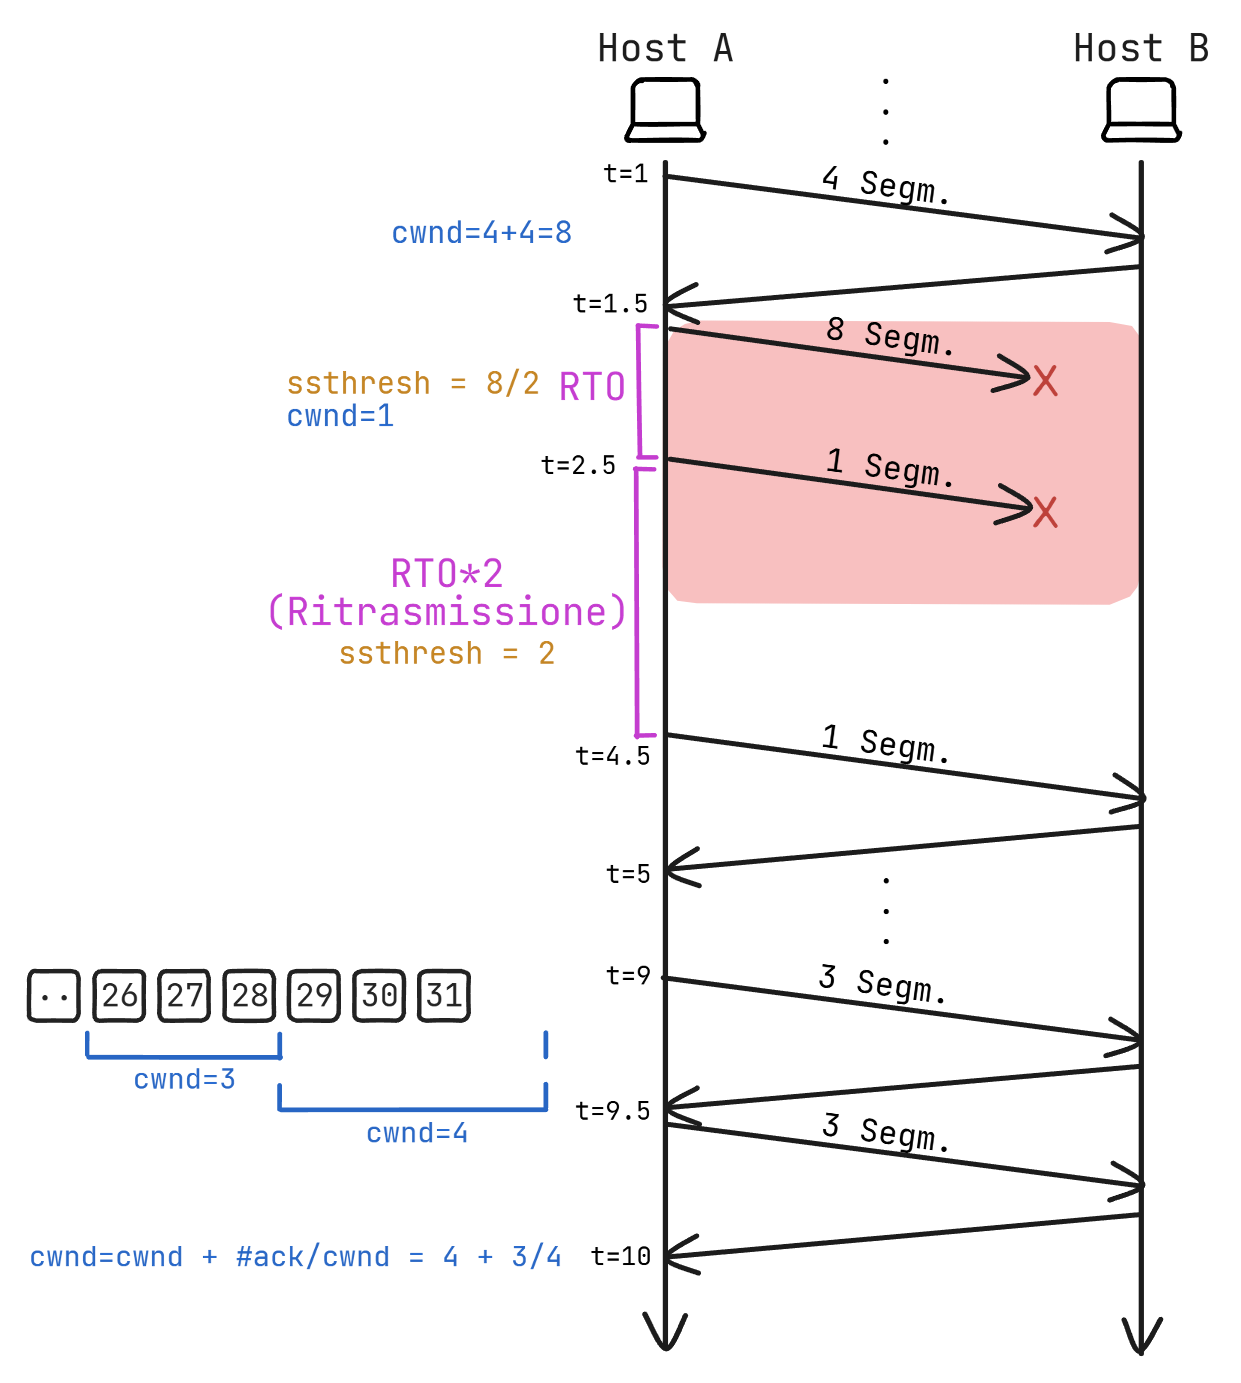
\includegraphics[width=1\textwidth]{../figures/es-tcp2}
\end{figure}

\subsection{Esercizio 3}
Abbiamo un'applicazione \( A \) che trasferisce \( 104000byte \) verso un'applicazione \( B \).
\[
\begin{aligned}
  MSS &= 1200 \text{ byte}\\
  RCVWND_{\text{iniziale}} &= 24000 \text{ byte} \to \text{ costante}\\
  SSTHRESH &= RCVWND_{\text{iniziale}}\\
  RTT &= 0.5 \text{ secondi} \to \text{ costante}\\
  RTO &= 2 \cdot RTT \to \text{ raddoppia in caso di perdite consecutive}\\
  \text{Down di rete} &= [3.5 \to 4.5],[6.5 \to 10.5]
\end{aligned}
\] 

\subsubsection{Risoluzione}
Il numero di pacchetti inviati è:
\[
  \begin{aligned}
    \frac{104000}{1200} &= 87 \text{ segmenti}\\
    RCVWND_{\text{iniziale}} &= \frac{24000}{1200} = 20\\
    SSTHRESH &= 20 \text{ segmenti}
  \end{aligned}
\] 
L'evoluzione della finestra di congestione è la seguente:
\begin{figure}[H]
  \centering
  \begin{tikzpicture}
    \def\xscale{1/2.8}
    \def\yscale{1/2}

    \def\yaxis{20}
    \def\xaxis{30}
    \draw[->] (0,-0.2) -- (0,\yaxis*\yscale+1*\yscale) node[left] {\( w \)};
    \draw[->] (-0.2,0) -- (\xaxis*\xscale+1*\xscale,0) node[below] {\( t \)};

    \def\rcvwnd{20}

    % rcvwnd & ssthresh
    \draw[red] (0,\rcvwnd*\yscale) node[above right] {\texttt{rcvwnd}} -- (\xaxis*\xscale+1*\xscale,\rcvwnd*\yscale);
    \draw[orange] (0,20*\yscale) node[below right] {\texttt{ssthresh}} -- (5*\xscale,20*\yscale)
      -- (9*\xscale,20*\yscale) -- (9*\xscale,10*\yscale)
      -- (15*\xscale,10*\yscale) -- (15*\xscale,5*\yscale)
      -- (19*\xscale,5*\yscale) -- (19*\xscale,2*\yscale)
      -- (\xaxis*\xscale+1*\xscale,2*\yscale);

    % Down
    \fill[red,opacity=0.2] (7*\xscale,0) rectangle (9*\xscale,\rcvwnd*\yscale);
    \fill[red,opacity=0.2] (13*\xscale,0) rectangle (21*\xscale,\rcvwnd*\yscale);

    \fill[blue] (0,1*\yscale) circle (0.05) node[scale=0.1] (1) {};
    \fill[blue] (1*\xscale,2*\yscale) circle (0.05) node[scale=0.1] (2) {};
    \fill[blue] (2*\xscale,4*\yscale) circle (0.05) node[scale=0.1] (3) {};
    \fill[blue] (3*\xscale,8*\yscale) circle (0.05) node[scale=0.1] (4) {};
    \fill[blue] (4*\xscale,16*\yscale) circle (0.05) node[scale=0.1] (5) {};
    \fill[blue] (5*\xscale,20*\yscale) circle (0.05) node[scale=0.1] (6) {};
    \fill[blue] (6*\xscale,20*\yscale) circle (0.05) node[scale=0.1] (7) {};
    \fill[blue] (7*\xscale,20*\yscale) circle (0.05) node[right,red] {\( \times \)} node[scale=0.1] (8) {};
    \draw[blue] (1) -- (2) -- (3) -- (4) -- (5) -- (6) -- (7) -- (8);

    % Loss
    \draw[purple,dashed] (7*\xscale,20*\yscale) -- (9*\xscale,20*\yscale) node[above] {\texttt{RTO}} -- (9*\xscale,1*\yscale);

    \fill[blue] (9*\xscale,1*\yscale) circle (0.05) node[scale=0.1] (9) {};
    \fill[blue] (10*\xscale,2*\yscale) circle (0.05) node[scale=0.1] (10) {};
    \fill[blue] (11*\xscale,4*\yscale) circle (0.05) node[scale=0.1] (11) {};
    \fill[blue] (12*\xscale,8*\yscale) circle (0.05) node[scale=0.1] (12) {};
    \fill[blue] (13*\xscale,10*\yscale) circle (0.05) node[right,red] {\( \times \)} node[scale=0.1] (13) {};
    \draw[blue] (9) -- (10) -- (11) -- (12) -- (13);

    % Loss
    \draw[purple,dashed] (13*\xscale,10*\yscale) -- (15*\xscale,10*\yscale) -- (15*\xscale,1*\yscale);

    \fill[blue] (15*\xscale,1*\yscale) circle (0.05) node[right,red] {\( \times \)} node[scale=0.1] (14) {};

    % Loss
    \draw[purple,dashed] (15*\xscale,1*\yscale) -- (19*\xscale,1*\yscale);

    \fill[blue] (19*\xscale,1*\yscale) circle (0.05) node[right,red] {\( \times \)} node[scale=0.1] (15) {};

    % Loss
    \draw[purple,dashed] (19*\xscale,1*\yscale) -- (27*\xscale,1*\yscale);

    \fill[blue] (27*\xscale,1*\yscale) circle (0.05) node[scale=0.1] (16) {};
    \fill[blue] (28*\xscale,2*\yscale) circle (0.05) node[scale=0.1] (17) {};
    \draw[blue] (16) -- (17);

    % End
    \draw[dashed] (28*\xscale,2*\yscale) -- (28*\xscale,0) node[below,align=center,scale=0.8] {Fine\\trasmissione};

    % Ticks
    \foreach \x in {1,2,...,\xaxis}
    \draw (\x*\xscale,-0.1) -- (\x*\xscale,0.1);

    \foreach \y in {1,2,...,\yaxis}
    \draw (0,\y*\yscale) -- (0.1,\y*\yscale);

    \foreach \y in {1,2,4,8,...,\yaxis}
    \draw (-0.1,\y*\yscale) -- (0.1,\y*\yscale) node[left=0.2] {\y};

    \node[below,scale=0.6] at (1*\xscale,0) {0.5};
    \node[below,scale=0.6] at (2*\xscale,-0.1) {1};
    \node[below,scale=0.6] at (7*\xscale,-0.1) {3.5};
    \node[below,scale=0.6] at (9*\xscale,-0.1) {4.5};
    \node[below,scale=0.6] at (13*\xscale,-0.1) {6.5};
    \node[below,scale=0.6] at (21*\xscale,-0.1) {10.5};

    \draw[green!50!black] (0,-0.2) -- ++(0,-0.2) -- ++(1*\xscale,0)
      node[midway,below] {RTT} -- ++(0,0.2);
  \end{tikzpicture}
  \caption{Andamento di \texttt{cwnd} in funzione del tempo}
\end{figure}
\noindent
Il numero di segmenti trasmessi è:
\[
  \#seg = 1+2+4+8+16+20+20+\cancel{16}+1+2+4+8+\cancel{1}+\cancel{1}+\cancel{1}+1
\] 
\[
= 87
\] 

\subsection{Esercizio 4}
Un'applicazione \( A \) trasferisce \( 104400byte \) verso un'applicazione \( B \).
\[
\begin{aligned}
  MSS &= 1200 \text{ byte}\\
  RCVWND_{\text{iniziale}} &= 9600 \text{ byte}\\
  SSTHRESH &= RCVWND_{\text{iniziale}}\\
  RTT &= 1 \text{ secondo} \to \text{ costante}\\
  RTO &= 2 \cdot RTT \to \text{ raddoppia in caso di perdite consecutive}\\
  \text{Down di rete} &= [11.5 \to 12.5]
\end{aligned}
\]
A partire dall'istante \( t_a > 4\,sec \) la destinazione annuncia una
\[
  RCVWND = 14400\,byte
\]
A partire dall'istante \( t_b > 9\,sec \) la destinazione annuncia una
\[
  RCVWND = 7200\,byte
\]

\vspace{1em}
\noindent
Bisogna tenere in considerazione il ritardo di ricezione dell'annuncio della nuova
\( RCVWND \) 

\subsubsection{Risoluzione}
Il numero di segmenti da trasmettere sono:
\[
  \frac{104400}{1200} = 87 \text{ segmenti}
\]
\[
  RCVWND_{\text{iniziale}} = \frac{9600}{1200} = 8 \text{ segmenti}
\]
\[
  \begin{aligned}
    SSTHRESH &= 8 \text{ segmenti}\\
    \quad t^{dst}_a > 4 &= 12 \text{ segmenti}\\
    \quad t^{dst}_b > 9 &= 6 \text{ segmenti}
  \end{aligned}
\] 
L'evoluzione della finestra di congestione è la seguente:
\begin{figure}[H]
  \centering
  \begin{tikzpicture}
    \def\xscale{1/1.7}
    \def\yscale{1/1.7}

    \def\yaxis{12}
    \def\xaxis{17}
    \draw[->] (0,-0.2) -- (0,\yaxis*\yscale+1*\yscale) node[left] {\( w \)};
    \draw[->] (-0.2,0) -- (\xaxis*\xscale+1*\xscale,0) node[below] {\( t \)};

    % rcvwnd & ssthresh
    \draw[red] (0,8*\yscale) node[above right] {\texttt{rcvwnd}}
      -- (5*\xscale,8*\yscale) -- (5*\xscale,12*\yscale)
      -- (10*\xscale,12*\yscale) -- (10*\xscale,6*\yscale)
      -- (\xaxis*\xscale+1*\xscale,6*\yscale);
    \draw[orange] (0,8*\yscale) node[below right] {\texttt{ssthresh}} -- (5*\xscale,8*\yscale)
      -- (13*\xscale,8*\yscale) -- (13*\xscale,3*\yscale)
      -- (\xaxis*\xscale+1*\xscale,3*\yscale);

    % Down
    \fill[red,opacity=0.2] (11.5*\xscale,0) rectangle (12.5*\xscale,6*\yscale);

    \fill[blue] (0,1*\yscale) circle (0.05) node[scale=0.1] (1) {};
    \fill[blue] (1*\xscale,2*\yscale) circle (0.05) node[scale=0.1] (2) {};
    \fill[blue] (2*\xscale,4*\yscale) circle (0.05) node[scale=0.1] (3) {};
    \fill[blue] (3*\xscale,8*\yscale) circle (0.05) node[scale=0.1] (4) {};
    \fill[blue] (4*\xscale,8*\yscale) circle (0.05) node[scale=0.1] (5) {};
    \fill[blue] (5*\xscale,9*\yscale) circle (0.05) node[scale=0.1] (6) {};
    \fill[blue] (6*\xscale,10*\yscale) circle (0.05) node[scale=0.1] (7) {};
    \fill[blue] (7*\xscale,11*\yscale) circle (0.05) node[scale=0.1] (8) {};
    \fill[blue] (8*\xscale,12*\yscale) circle (0.05) node[scale=0.1] (9) {};
    \fill[blue] (9*\xscale,12*\yscale) circle (0.05) node[scale=0.1] (10) {};
    \fill[blue] (10*\xscale,6*\yscale) circle (0.05) node[scale=0.1] (11) {};
    \fill[blue] (11*\xscale,6*\yscale) circle (0.05) node[right,red] {\( \times \)} node[scale=0.1] (12) {};
    \draw[blue] (1) -- (2) -- (3) -- (4) -- (5) -- (6) -- (7) -- (8) -- (9) -- (10) -- (11) -- (12);

    % Loss
    \draw[purple,dashed] (11*\xscale,6*\yscale) -- (13*\xscale,6*\yscale) node[above] {\texttt{RTO}} -- (13*\xscale,1*\yscale);

    \fill[blue] (13*\xscale,1*\yscale) circle (0.05) node[scale=0.1] (13) {};
    \fill[blue] (14*\xscale,2*\yscale) circle (0.05) node[scale=0.1] (14) {};
    \fill[blue] (15*\xscale,3*\yscale) circle (0.05) node[scale=0.1] (15) {};
    \fill[blue] (16*\xscale,3*\yscale + 1/3*\yscale) circle (0.05) node[scale=0.1] (16) {}
      node[above,scale=0.8] {\( 3 + \frac{1}{3} \)};
    \draw[blue] (13) -- (14) -- (15) -- (16);

    % End
    \draw[dashed] (16*\xscale,3*\yscale + 1/3*\yscale) -- (16*\xscale,0) node[below,align=center,scale=0.8] {Fine\\trasmissione};

    % Ticks
    \foreach \x in {1,2,...,\xaxis}
    \draw (\x*\xscale,-0.1) -- (\x*\xscale,0.1);

    \foreach \y in {1,2,...,\yaxis}
    \draw (0,\y*\yscale) -- (0.1,\y*\yscale);

    \foreach \y in {1,2,4,8,...,\yaxis}
    \draw (-0.1,\y*\yscale) -- (0.1,\y*\yscale) node[left=0.2] {\y};

    \node[below right,scale=0.6] at (1*\xscale,-0.1) {1};
    \node[below,scale=0.6] at (2*\xscale,-0.1) {2};
    \node[below,scale=0.6] at (11.5*\xscale,-0.1) {11.5};
    \node[below,scale=0.6] at (12.5*\xscale,-0.1) {12.5};

    \draw[green!50!black] (0,-0.2) -- ++(0,-0.2) -- ++(1*\xscale,0)
      node[midway,below] {RTT} -- ++(0,0.2);
  \end{tikzpicture}
  \caption{Andamento di \texttt{cwnd} in funzione del tempo}
\end{figure}
\noindent
Il numero di segmenti trasmessi è:
\[
  \#seg = 1+2+4+8+8+9+10+11+12+12+6+\cancel{4}+1+2+\stackrel{1}{\cancel{3}} = 87
\]
Un'altra possibile rappresentazione è la seguente:
\begin{figure}[H]
  \centering
  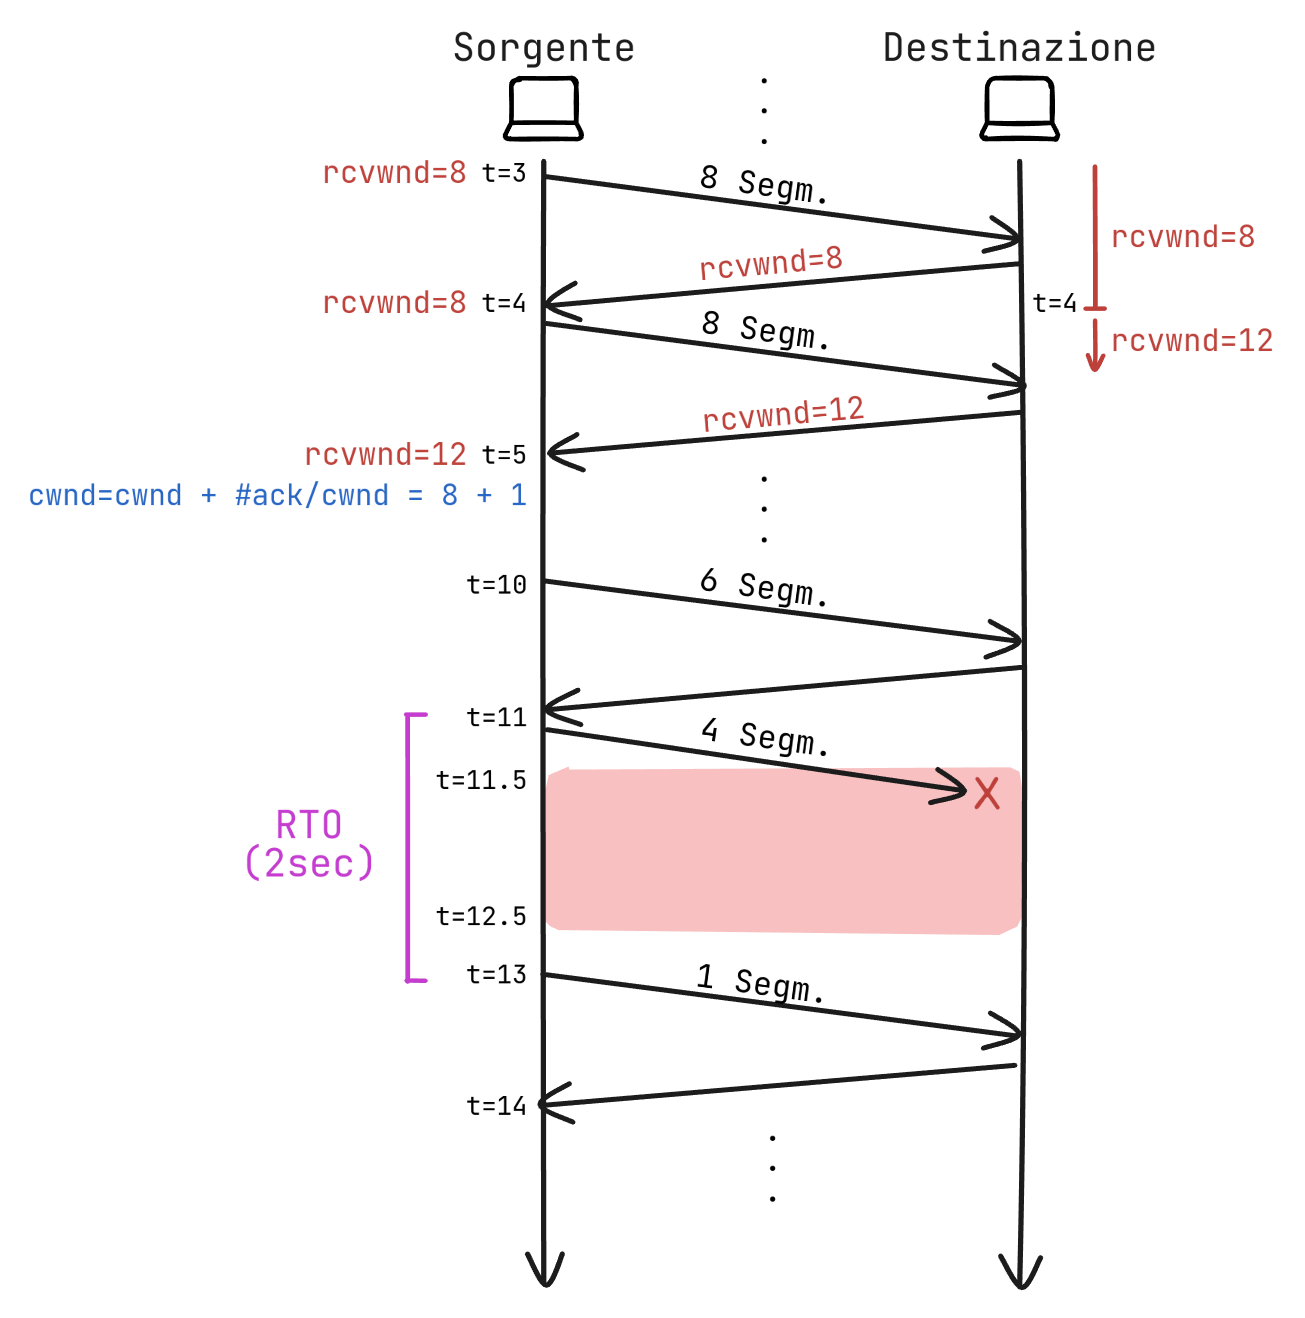
\includegraphics[width=1\textwidth]{../figures/es-tcp4}
\end{figure}

\vspace{1em}
\noindent
Se al posto di perdere il pacchetto si fosse perso il riscontro, avremmo avuto la seguente
rappresentazione:
\begin{figure}[H]
  \centering
  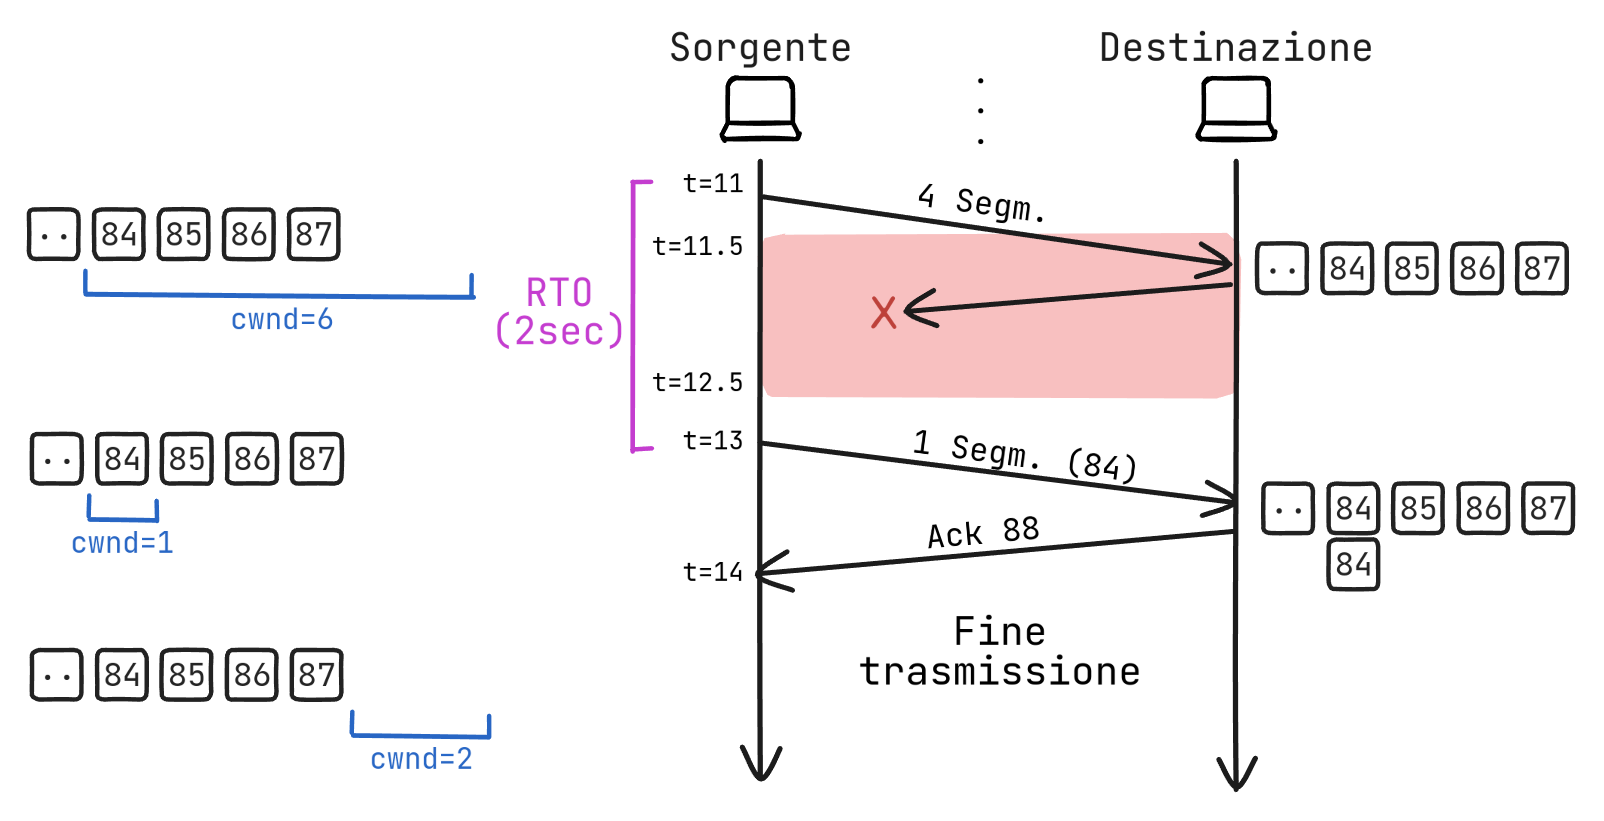
\includegraphics[width=1\textwidth]{../figures/es-tcp4.1}
\end{figure}
\noindent
Anche questa rappresentazione è corretta, in quanto il numero di segmenti trasmessi è
sempre 87.

\subsection{Esercizio 5}
Un applicazione \( A \) trasferisce \( 77500 \,byte\) verso un'applicazione \( B \).
\[
\begin{aligned}
  MSS &= 1250 \,byte\\
  RCVWND_{\text{iniziale}} &= 10000 \,byte\\
  SSTHRESH &= RCVWND_{\text{iniziale}}\\
  RTT &= 1 \,second0 \to \text{costante}\\
  RTO &= 2 \cdot RTT \to \text{raddoppia in caso di perdite consecutive}\\
  \text{Down di rete} &= [8 \to 10],[13.5 \to 14.5]
\end{aligned}
\]
A partire dall'istante \( t_a > 4\,sec \) la destinazione annuncia una
\[
  RCVWND = 17500\,byte
\]
A partire dall'istante \( t_b > 8\,sec \) la destinazione annuncia una
\[
  RCVWND = 12500\,byte
\] 

\subsubsection{Risoluzione}
Il numero di segmenti da trasmettere sono:
\[
  \frac{77500}{1250} = 62 \text{ segmenti}
\]
\[
  RCVWND_{\text{iniziale}} = \frac{10000}{1250} = 8 \text{ segmenti}
\]
\[
  \begin{aligned}
    SSTHRESH &= 8 \text{ segmenti}\\
    \quad t^{dst}_a > 4 \quad RCVWND &= 14 \text{ segmenti}\\
    \quad t^{dst}_b > 8 \quad RCVWND &= 10 \text{ segmenti}
  \end{aligned}
\]
\begin{figure}[H]
  \centering
  \begin{tikzpicture}
    \def\xscale{1/1.7}
    \def\yscale{1/1.7}

    \def\yaxis{14}
    \def\xaxis{17}
    \draw[->] (0,-0.2) -- (0,\yaxis*\yscale+1*\yscale) node[left] {\( w \)};
    \draw[->] (-0.2,0) -- (\xaxis*\xscale+1*\xscale,0) node[below] {\( t \)};

    % rcvwnd & ssthresh
    \draw[red] (0,8*\yscale) node[above right] {\texttt{rcvwnd}}
      -- (5*\xscale,8*\yscale) -- (5*\xscale,14*\yscale)
      -- (9*\xscale,14*\yscale) -- (9*\xscale,10*\yscale)
      -- (\xaxis*\xscale+1*\xscale,10*\yscale);
    \draw[orange] (0,8*\yscale) node[below right] {\texttt{ssthresh}}
      -- (10*\xscale,8*\yscale) -- (10*\xscale,6*\yscale)
      -- (15*\xscale,6*\yscale) -- (15*\xscale,3*\yscale)
      -- (\xaxis*\xscale+1*\xscale,3*\yscale);

    % Down
    \fill[red,opacity=0.2] (8*\xscale,0) rectangle (10*\xscale,\yaxis*\yscale);
    \fill[red,opacity=0.2] (13.5*\xscale,0) rectangle (14.5*\xscale,\yaxis*\yscale);

    \fill[blue] (0,1*\yscale) circle (0.05) node[scale=0.1] (1) {};
    \fill[blue] (1*\xscale,2*\yscale) circle (0.05) node[scale=0.1] (2) {};
    \fill[blue] (2*\xscale,4*\yscale) circle (0.05) node[scale=0.1] (3) {};
    \fill[blue] (3*\xscale,8*\yscale) circle (0.05) node[scale=0.1] (4) {};
    \fill[blue] (4*\xscale,8*\yscale) circle (0.05) node[scale=0.1] (5) {};
    \fill[blue] (5*\xscale,9*\yscale) circle (0.05) node[scale=0.1] (6) {};
    \fill[blue] (6*\xscale,10*\yscale) circle (0.05) node[scale=0.1] (7) {};
    \fill[blue] (7*\xscale,11*\yscale) circle (0.05) node[scale=0.1] (8) {};
    \fill[blue] (8*\xscale,12*\yscale) circle (0.05) node[scale=0.1] (9) {} node[right,red] {\( \times \)};
    \draw[blue] (1) -- (2) -- (3) -- (4) -- (5) -- (6) -- (7) -- (8) -- (9);

    % Loss
    \draw[purple,dashed] (8*\xscale,12*\yscale) -- (10*\xscale,12*\yscale) node[above]
      {\texttt{RTO}} -- (10*\xscale,1*\yscale);


    \fill[blue] (10*\xscale,1*\yscale) circle (0.05) node[scale=0.1] (10) {};
    \fill[blue] (11*\xscale,2*\yscale) circle (0.05) node[scale=0.1] (11) {};
    \fill[blue] (12*\xscale,4*\yscale) circle (0.05) node[scale=0.1] (12) {};
    \fill[blue] (13*\xscale,6*\yscale) circle (0.05) node[scale=0.1] (13) {} node[right,red] {\( \times \)};
    \draw[blue] (10) -- (11) -- (12) -- (13);

    % Loss
    \draw[purple,dashed] (13*\xscale,6*\yscale) -- (15*\xscale,6*\yscale) -- (15*\xscale,1*\yscale);


    \fill[blue] (15*\xscale,1*\yscale) circle (0.05) node[scale=0.1] (14) {};
    \fill[blue] (16*\xscale,2*\yscale) circle (0.05) node[scale=0.1] (15) {};
    \fill[blue] (17*\xscale,3*\yscale) circle (0.05) node[scale=0.1] (16) {};
    \draw[blue] (14) -- (15) -- (16);

    % End
    \draw[dashed] (17*\xscale,2*\yscale+1/2*\yscale) -- (17*\xscale,0) node[below,align=center,scale=0.8] {Fine\\trasmissione};

    % Ticks
    \foreach \x in {1,2,...,\xaxis}
    \draw (\x*\xscale,-0.1) -- (\x*\xscale,0.1);

    \foreach \y in {1,2,...,\yaxis}
    \draw (0,\y*\yscale) -- (0.1,\y*\yscale);

    \foreach \y in {1,2,4,8,...,\yaxis}
    \draw (-0.1,\y*\yscale) -- (0.1,\y*\yscale) node[left=0.2] {\y};

    \node[below right,scale=0.6] at (1*\xscale,-0.1) {1};
    \node[below,scale=0.6] at (2*\xscale,-0.1) {2};
    \node[below,scale=0.6] at (8*\xscale,-0.1) {8};
    \node[below,scale=0.6] at (10*\xscale,-0.1) {10};
    \node[below,scale=0.6] at (13.5*\xscale,-0.1) {13.5};
    \node[below,scale=0.6] at (14.5*\xscale,-0.1) {14.5};

    \draw[green!50!black] (0,-0.2) -- ++(0,-0.2) -- ++(1*\xscale,0)
      node[midway,below] {RTT} -- ++(0,0.2);
  \end{tikzpicture}
  \caption{Andamento di \texttt{cwnd} in funzione del tempo}
\end{figure}
\noindent
Il numero di segmenti trasmessi è:
\[
  \#seg = 1+2+4+8+8+9+10+11+\cancel{12}+1+2+4+\cancel{6}+1+\stackrel{1}{\cancel{2}} = 62
\]

\end{document}
